\newpage
\section{Картотека пациентов}

В \tmis ~для каждого пациента заводится регистрационная карточка, которая содержит всю персональную информацию о пациенте. Она регистрируется в системе при первичном обращении пациента в МУ и выполняет функцию амбулаторной карты пациента. При всех последующих обращениях осуществляется поиск ранее зарегистрированной карточки пациента и привязка к ней очередного случая обращения. В случае изменения каких-либо персональных данных пациента, регистрационную карточку можно отредактировать. 

Таким образом, при работе с \tmis~персональные данные пациента вносятся в систему один раз, а медицинские записи добавляются при каждом обращении. Благодаря данному механизму значительно упрощается процесс получение врачом медицинской информации о предыдущих случаях обращения пациента.

Совокупность регистрационных карточек пациентов, случаев их обращений в ЛПУ и результатов обращений называется картотекой пациентов. Для доступа к картотеке пациентов необходимо нажать кнопку \btn{Обслуживание пациентов} вверху страницы на панели управления, либо нажать на блок \dm{Обслуживание пациентов} на главной странице системы (Рисунок \ref{img_gen_main}). Будет осуществлен переход на страницу \dm{Обслуживание пациентов} (Рисунок \ref{img_cl_find}). Здесь можно найти карточку пациента или зарегистрировать нового пациента, просмотреть предварительные записи на прием и данные обращений пациента, а так же зарегистрировать новые.

\begin{figure}[ht]\centering
 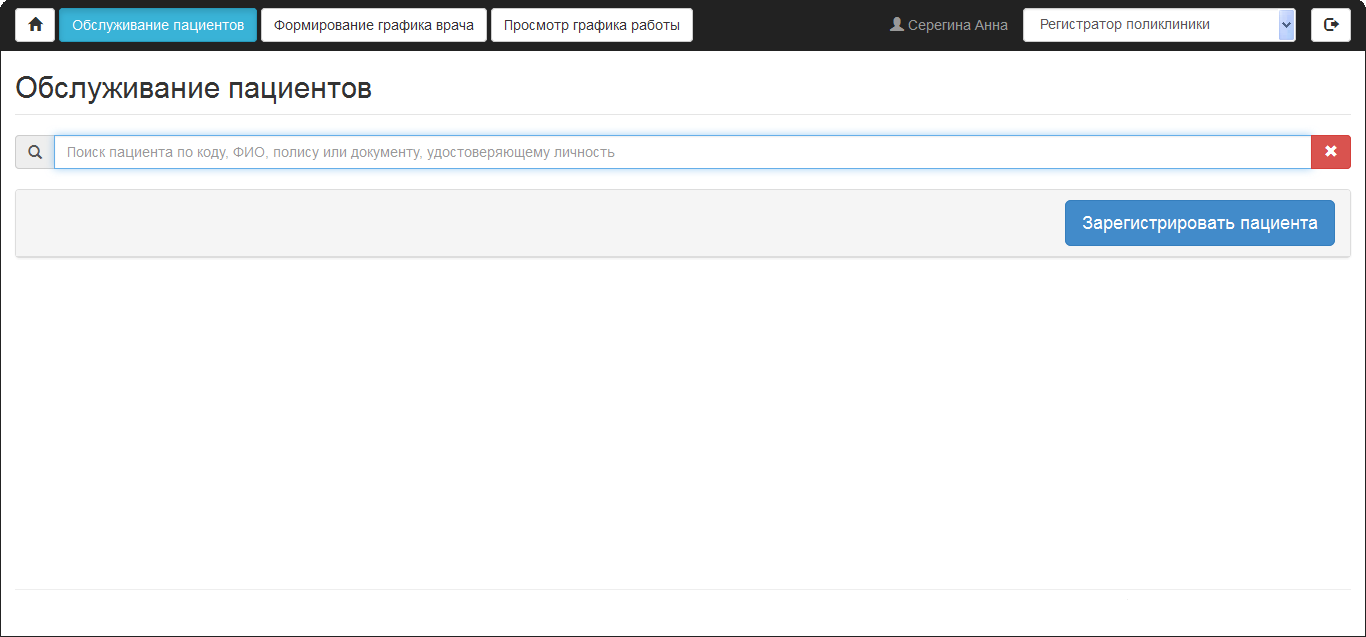
\includegraphics[width = 1\textwidth ,keepaspectratio]{cl_find}
 \caption{Страница поиска и обслуживания пациентов}
 \label{img_cl_find}
\end{figure} 

\subsection{Поиск регистрационной карточки пациента} \label{cl_find}

В верхней части страницы находится поле для задания параметров поиска пациентов. В него в произвольном порядке можно ввести фамилию, имя, отчество, код пациента, номера его полиса ОМС или документа, удостоверяющего личность. Во время ввода символов в поле поиска будет автоматически производиться фильтрация пациентов на основе введенных данных. После прекращения ввода данных в поле поиска, на экране появится список найденных пациентов (Рисунок \ref{img_cl_findrez}).
 
\begin{figure}[ht]\centering
 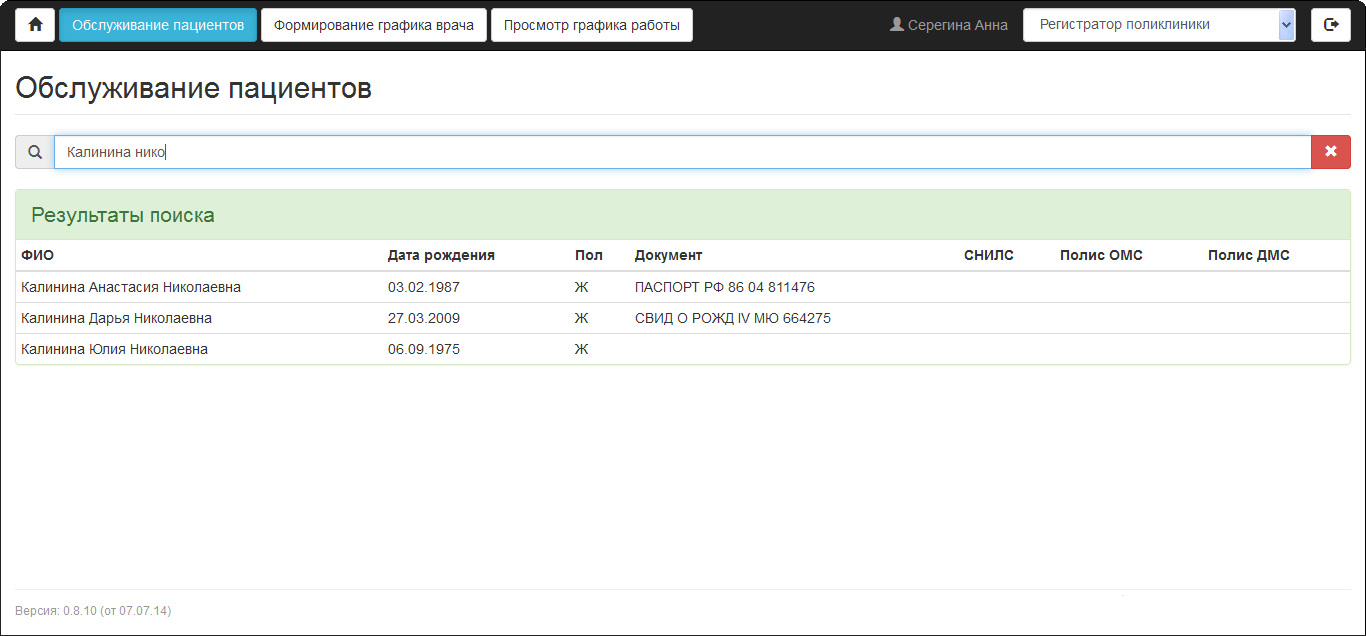
\includegraphics[width = 1\textwidth ,keepaspectratio]{cl_findrez}
 \caption{Результаты поиска пациентов}
 \label{img_cl_findrez}
\end{figure} 

\begin{vnim}
Нажатие клавиши \keys{Enter} в поле поиска приводит к сбросу параметров фильтрации. В результате, на экране отобразится полный список пациентов.
\end{vnim}

Если по заданным параметрам не будет найдено ни одного пациента, по под полем поиска появится сообщение <<Пациент не найден в базе данных>> и останется доступной кнопка \btn{Зарегистрировать пациента}.

\subsection{Регистрационная карточка пациента} \label{cl_card}

Регистрационная карточка пациента содержит всю персональную информацию о пациенте: его фамилию, имя, отчество, дату рождения, адрес, сведения о документах пациента, его страховых полисах, льготах, занятости и т.д. Вся эта информация должна вводиться регистратором с первичных документов пациента при его первом обращении в ЛПУ. В момент регистрации пациента ему присваивается уникальный код, по которому его регистрационную карточку можно быстро найти в картотеке пациентов.

Для регистрации нового пациента необходимо нажать кнопку \btn{Зарегистрировать пациента} на странице обслуживания пациентов (Рисунок \ref{img_cl_find}). 

Регистрационная карточка пациента имеет вид, приведенный на рисунке \ref{img_cl_card}. Карточка содержит большое количество разделов. Для перехода к определенному разделу можно щелкнуть левой кнопкой мыши по названию соответствующего раздела в левой части страницы либо воспользоваться полосой прокрутки и найти раздел самостоятельно.  

\begin{figure}[ht]\centering
 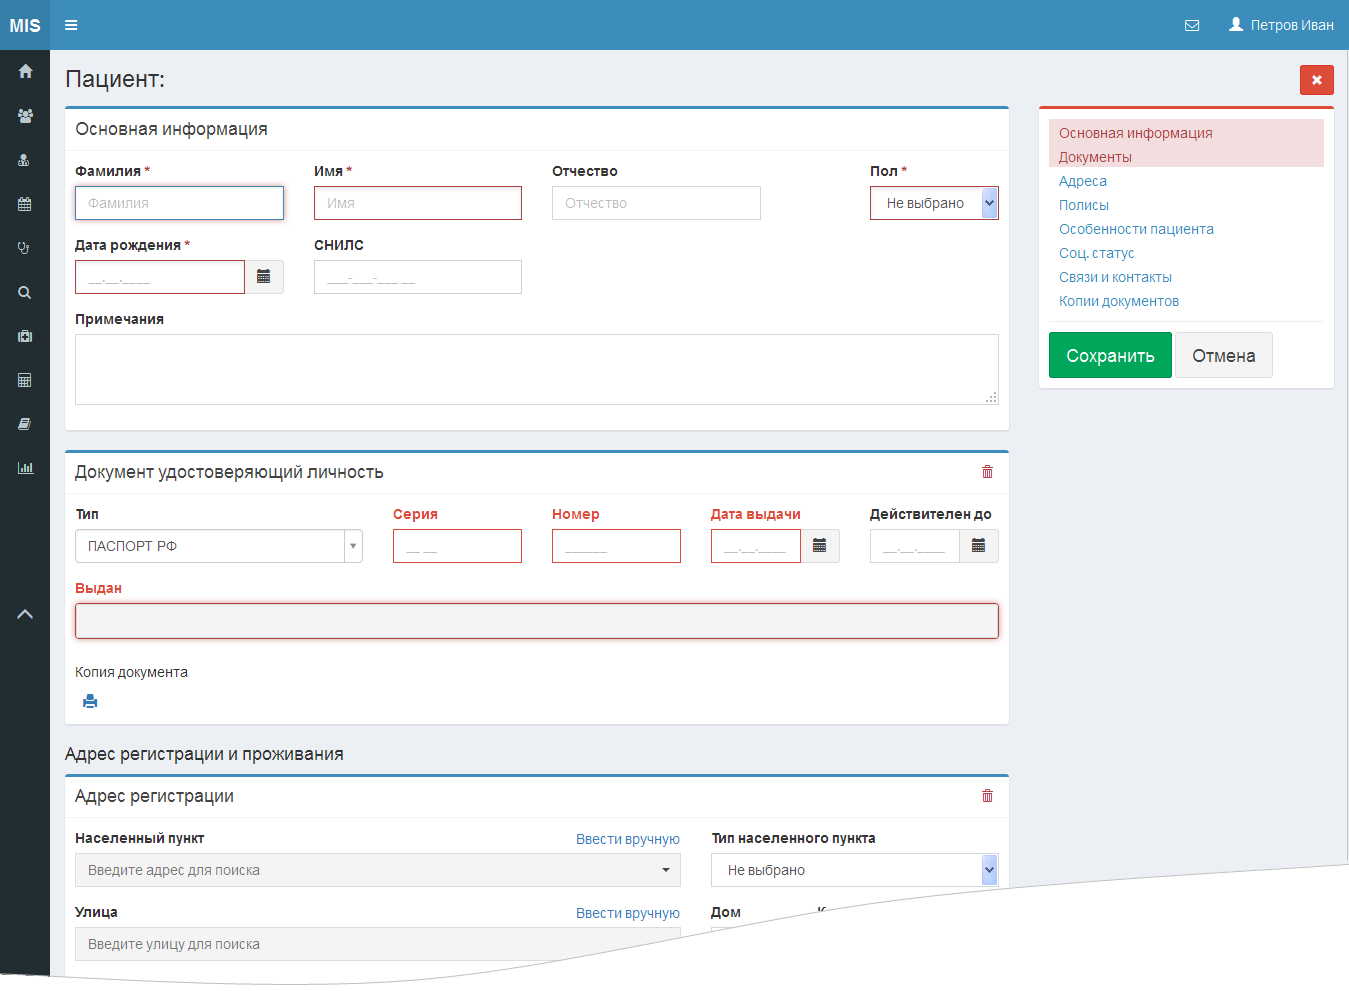
\includegraphics[width = 1\textwidth ,keepaspectratio]{cl_card}
 \caption{Регистрационная карточка пациента}
 \label{img_cl_card}
\end{figure} 

\subsubsection{Блок <<Основная информация>>}

Поля \dm{Фамилия}, \dm{Имя}, \dm{Дата рождения} и \dm{Пол} в карточке регистрации пациента являются обязательными для заполнения. Они помечены символом <<*>> красного цвета.

Поля, задающие даты, могут заполняться с клавиатуры или выбираться из календаря. При заполнении с клавиатуры дата вводится в формате <<ДД.ММ.ГГГГ>>. Разделительные точки при этом вводить необязательно, они будут вставлены автоматически.

Значение поля \dm{Пол} может вводиться с клавиатуры или выбираться из списка с помощью мыши. 

В поле \dm{СНИЛС} достаточно ввести только цифры, разделительные тире будут вставлены автоматически. При вводе СНИЛС автоматически проводится проверка корректности введенного значения. В случае, если введенное значение не прошло проверку, поле будет выделено красным цветом и появится подсказка <<Введен невалидный СНИЛС>>. Сохранение карточки пациента с неверным СНИЛС невозможно.

В поле \dm{Примечание} можно внести дополнительные сведения о пациенте, для которых не предусмотрено отдельных полей в карточке пациента. 
 
\subsubsection{Блок <<Документ удостоверяющий личность>>}

В данном блоке указываются данные документа, удостоверяющего личность пациента. Как правило, для детей таким документом является свидетельство о рождении, а для взрослых – паспорт, однако, возможны и другие варианты. \dm{Тип документа} выбирается из справочника. В зависимости выбранного типа документа, определяется набор реквизитов документа, необходимых для заполнения. Обязательные для заполнения поля подсвечиваются красным цветом. 

Для большинства типов документов требуется указать серию, номер, дату выдачи, срок действия и кем был выдан документ. В поле \dm{Выдан} данные можно ввести с клавиатуры или выбрать из раскрывающегося списка. В случае если какие-то данные в документе не указаны (например, не все документы имеют номер серии или срок действия), соответствующие поля заполнять не нужно.

\subsubsection{Блок <<Адрес регистрации и проживания>>}

В регистрационной карточке существует возможность указания двух адресов для каждого пациента: адреса регистрации и адреса фактического проживания (Рисунок \ref{img_cl_adres}). 

\begin{figure}[ht]\centering
 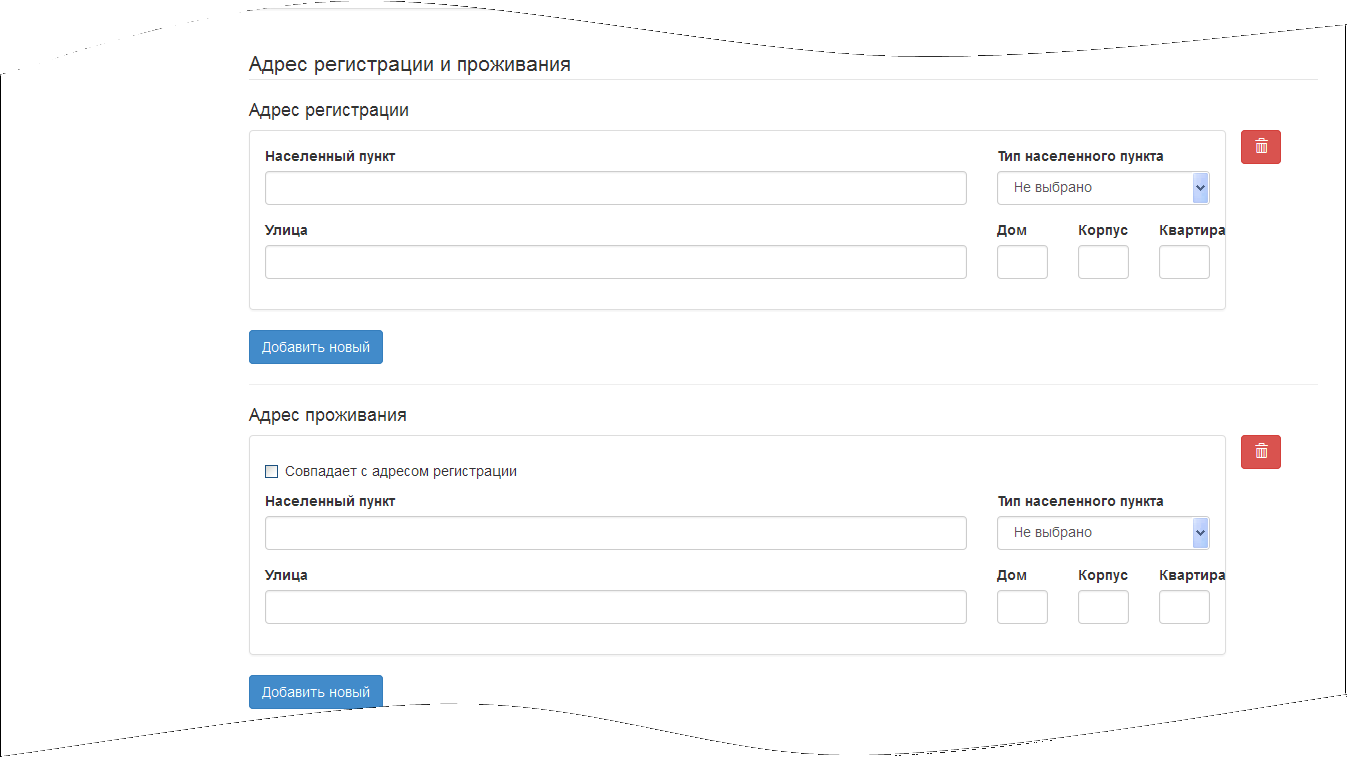
\includegraphics[width = 1\textwidth ,keepaspectratio]{cl_adres}
 \caption{Регистрационная карточка пациента. Блок ввода адреса регистрации.}
 \label{img_cl_adres}
\end{figure} 

Заполнение адреса рекомендуется выполнять с помощью всероссийского классификатора адресов КЛАДР. Поиск адреса по справочнику КЛАДР производится автоматически по мере ввода названия населенного пункта или улицы в соответствующее поле. Найденные значения появляются в раскрывающемся списке поля. Если в списке присутствует нужное название, то следует выбрать его, щелкнув по нему левой кнопкой мыши, либо переместить курсор на этот элемент списка с помощью клавиш со стрелками на клавиатуре и нажать клавишу \keys{Enter}.

Если для данных, внесенных в поля \dm{Населенный пункт} и \dm{Улица}, не найдены соответствия в справочнике КЛАДР, то поля будут считаться заполненными с ошибками. Они будут подсвечены красным цветом, а в верхней части блока появится сообщение об ошибке <<Введенный адрес не найден в справочнике адресов Кладр. Ввести адрес вручную?>> (Рисунок \ref{img_cl_adrf}). Сохранение карточки пациента при этом будет невозможно. 

\begin{figure}[ht]\centering
 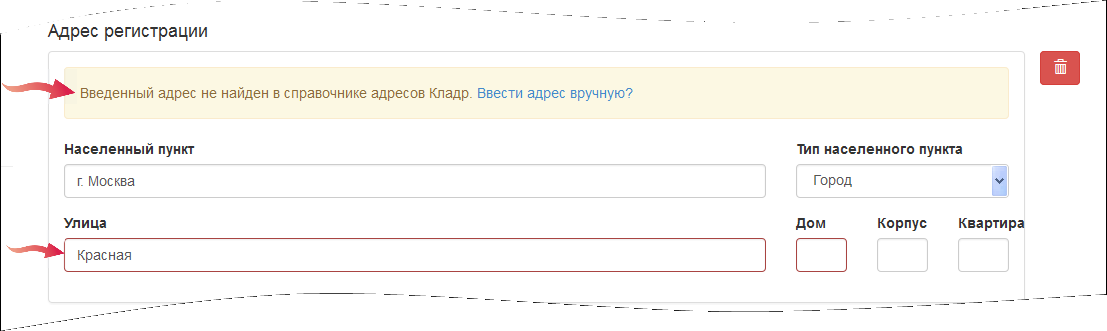
\includegraphics[width = 1\textwidth ,keepaspectratio]{cl_adrf}
 \caption{Регистрационная карточка пациента. Блок ввода адреса регистрации. Адрес не найден в справочнике КЛАДР}
 \label{img_cl_adrf}
\end{figure} 

В такой ситуации следует еще раз проверить правильность написания названий населенного пункта и улицы, попытаться использовать другое написание или альтернативные названия. Если и после этого найти соответствие в справочнике не удалось, можно нажать на фразу <<Ввести адрес вручную?>> в тексте сообщения об ошибке. Поля  \dm{Населенный пункт}, \dm{Улица}, \dm{Дом}, \dm{Корпус} и \dm{Квартира} при этом станут недоступными для редактирования, но появится новое поле \dm{В свободном виде} в нижней части блока, куда можно будет ввести адрес в виде текста. Проверка на соответствие справочнику Кладр производиться не будет (Рисунок \ref{img_cl_adrfree}). 

\begin{vnim}
Ввод адреса в свободной форме можно применять только в крайних случаях, при наличии веских причин. 
\end{vnim}

\begin{figure}[ht]\centering
 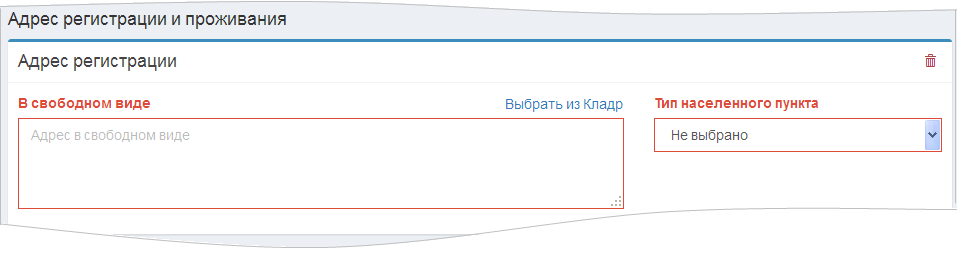
\includegraphics[width = 1\textwidth ,keepaspectratio]{cl_adrfree}
 \caption{Регистрационная карточка пациента. Блок ввода адреса регистрации. Ввод адреса в свободной форме}
 \label{img_cl_adrfree}
\end{figure}   

\begin{prim}
Для того, чтобы от свободного ввода снова вернуться к вводу адреса по справочнику КЛАДР, нужно щелкнуть в сообщении об ошибке вверху блока по фразе <<Выбрать из Кладр>>. При этом поле \dm{В свободном виде} исчезнет, а остальные поля снова станут доступны для редактирования.
\end{prim}

В полях ниже, аналогичным способом можно ввести адрес фактического проживания пациента. Если адрес фактического проживания совпадает с адресом регистрации, то в подразделе \dm{Адрес проживания} можно установить флажок \dm{Совпадает с адресом регистрации}. Тогда данные из подраздела \dm{Адрес регистрации} будут скопированы в соответствующие полях подраздела \dm{Адрес проживания}. Редактирование адреса проживания при этом становится недоступно. 
 
\subsubsection{Блок <<Медицинские полисы>>}
  
В подразделе \dm{Полис ОМС} (Рисунок \ref{img_cl_police}) указываются данные действующего полиса обязательного медицинского страхования. Необходимо указать тип полиса, его серию и номер, дату выдачи и срок действия. Поле \dm{Действителен до} может оставаться незаполненным, если срок действия полиса не ограничен. В строке \dm{СМО} требуется выбрать из справочника название СМО.

\begin{figure}[ht]\centering
 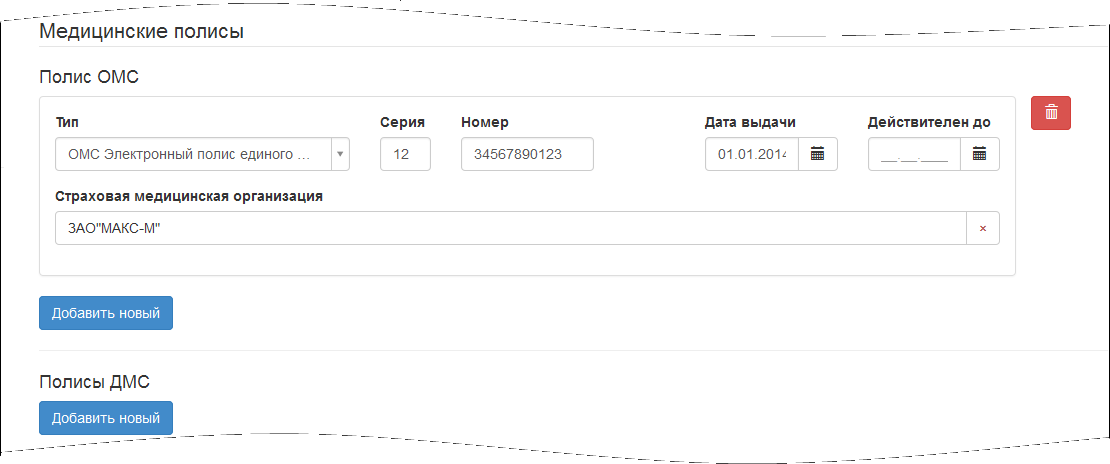
\includegraphics[width = 1\textwidth ,keepaspectratio]{cl_police}
 \caption{Регистрационная карточка пациента. Блок ввода полисов пациента.}
 \label{img_cl_police}
\end{figure}  

В подразделе \dm{Полис ДМС} по умолчанию отсутствуют данные. Для добавления полиса ДМС в карточку пациента необходимо нажать кнопку \btn{Добавить новый}. Появятся поля, аналогичные полям в подразделе \dm{Полис ОМС}, которые заполняются так же, как и в предыдущем подразделе, но хранят данные о действующем полисе ДМС пациента.

\begin{prim}
При изменении данных полиса или документа, удостоверяющего личность, ранее введенные данные не теряются. Все ранее зарегистрированные для пациента полисы  и документы, удостоверяющие личность, можно найти в блоке \dm{История изменений документов} (см.раздел \ref{cl_docs})
\end{prim}

\subsubsection{Блок <<Особенности пациента>>} 

Блок \dm{Особенности пациента} содержит жизненно-важные параметры, необходимые для оказания медицинской помощи (витальную информацию): группу крови, сведения об аллергии и медикаментозной непереносимости (Рисунок \ref{img_cl_osob}). 

\begin{figure}[ht]\centering
 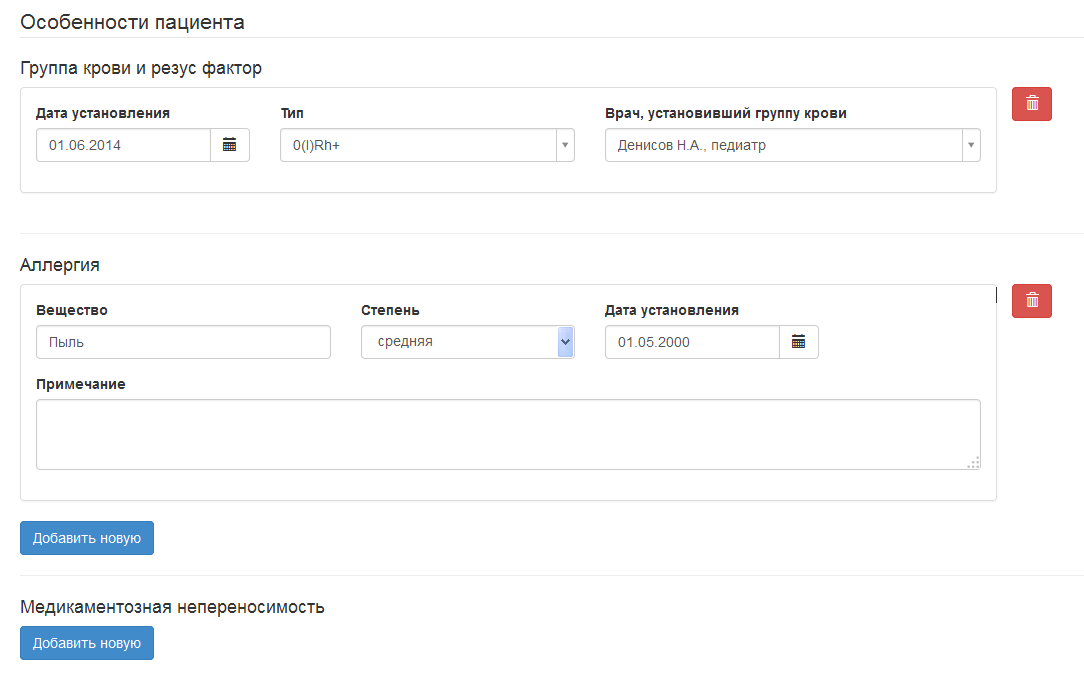
\includegraphics[width = 1\textwidth ,keepaspectratio]{cl_osob}
 \caption{Регистрационная карточка пациента. Блок <<Особенности пациента>>}
 \label{img_cl_osob}
\end{figure} 

Блок содержит 3 подраздела: 
\begin{itemize}
 \item Группа крови и резус фактор;
 \item Аллергия;
 \item Медикаментозная непереносимость.
\end{itemize}

По умолчанию поля для каждого из подразделов скрыты. Для добавления информации в какой-либо из подразделов необходимо нажать кнопку \btn{Добавить новую}. Тогда на странице появятся дополнительные поля для ввода информации соответствующего подраздела.

В подразделе \dm{Группа крови и резус-фактор} хранится информация о группе крови  и резусе пациента. Если группа крови известна на этапе регистрации пациента, то ее необходимо внести в регистрационную карточку пациента. В поле \dm{Дата установления} нужно указать дату установления группы крови, в поле \dm{Тип} группа крови и резус-фактор выбираются из справочника, в поле \dm{Врач, установивший группу крови} выбирается фамилия врача из справочника сотрудников, по умолчанию указывается фамилия текущего пользователя.

\begin{vnim}
Редактирование группы крови и резус-фактора после сохранения регистрационной карточки пациента становится невозможным.
\end{vnim}

Подразделы \dm{Аллергия} и \dm{Медикаментозная непереносимость} заполняются по одному и тому же принципу. В поле  \dm{Вещество (Препарат)} необходимо ввести описание аллергена, например <<пыль>> или <<доксициклин>>, в ячейке \dm{Степень} выбрать из списка степень аллергической реакции, в ячейке \dm{Дата установления} ввести дату установления аллергии (медикаментозной непереносимости), в поле \dm{Примечание}, можно указать дополнительные сведения относительно реакции. В каждом подразделе может содержаться любое количество записей. Поля \dm{Вещество (Препарат)}, \dm{Степень} и \dm{Дата установления} являются обязательными для заполнения. В случае их незаполнения, поля будут подсвечиваться красным цветом, сохранение регистрационной карточки пациента при этом будет невозможно.

\subsubsection{Блок <<Социальные статусы>>} 

В этом блоке можно внести ряд дополнительных сведений о пациенте, которые используются, в первую очередь для статистического учета (Рисунок \ref{img_cl_socst}): 
\begin{itemize}
 \item \dm{Инвалидность} -- данные о типе инвалидности пациента и документах, подтверждающих инвалидность.
 \item \dm{Занятость} -- сведения о занятости пациента.
 \item \dm{Гражданство}.
\end{itemize}

По умолчанию поля для каждого из подразделов скрыты. Для добавления информации в какой-либо из подразделов необходимо нажать кнопку \btn{Добавить инвалидность}, \btn{Добавить занятость}, \btn{Добавить гражданство} соответственно.

\begin{figure}[ht]\centering
 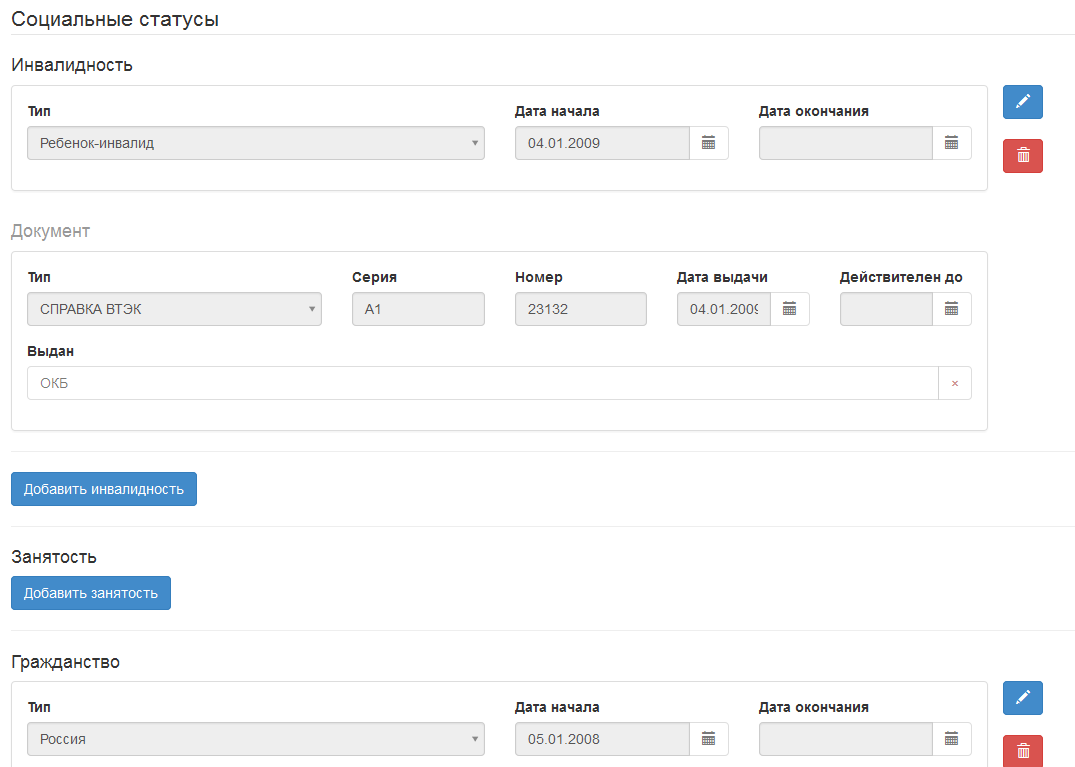
\includegraphics[width = 1\textwidth ,keepaspectratio]{cl_socst}
 \caption{Регистрационная карточка пациента. Блок <<Социальные статусы>>}
 \label{img_cl_socst}
\end{figure} 

При заполнении данных перечисленных подразделов необходимо выбрать значение в поле \dm{Тип} и указать дату в поле \dm{Дата начала}. Если настоящая дата установления статуса (например, гражданства) неизвестна, то можно указать текущую дату. Для инвалидности обязательно следует указывать настоящую дату в поле \dm{Дата начала}, а так же ввести данные документа, подтверждающего инвалидность.


\begin{prim}
Данные обо всех документах, подтверждающих инвалидность можно так же просмотреть в блоке \dm{История изменений документов}.
\end{prim}
 
\subsubsection{Блок <<Контактная информация и родственники>>}

В подраздел \dm{Связи с другими пациентами} содержит указатели на регистрационные карточки родственников пациента (Рисунок \ref{img_cl_contact}). 

\begin{vnim}
Для создания связи родственник должен быть зарегистрирован в \tmis.
\end{vnim}

\begin{figure}[ht!]\centering
 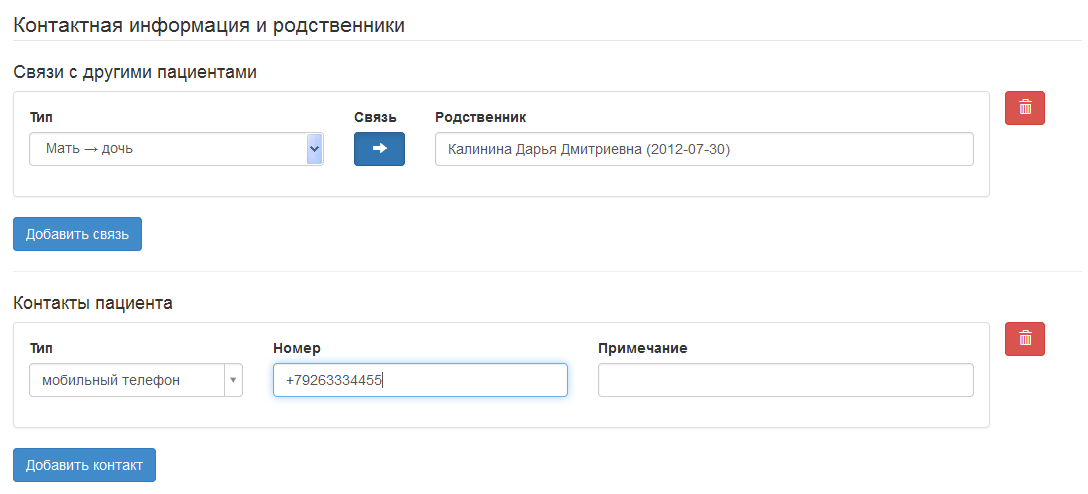
\includegraphics[width = 1\textwidth ,keepaspectratio]{cl_contact}
 \caption{Регистрационная карточка пациента. Блок <<Контактная информация и родственники>>}
 \label{img_cl_contact}
\end{figure} 

Для добавления связи необходимо нажать кнопку \btn{Добавить связь}, выбрать тип связи в поле \dm{Тип}, ввести в поле \dm{Родственник} фамилию, имя и отчество родственника пациента. По мере набора фамилии родственника в соответствующем поле, будет осуществляться поиск пациентов в БД. Результат поиска будет отображаться в раскрывающемся списке поля. Следует выбрать из этого списка нужного пациента. Если не будет найдено соответствия введенных данных с пациентами в БД, поле \dm{Родственник} будет подсвечено красным цветом. Сохранение регистрационной карточки пациента при этом будет невозможно.

Возможен ввод нескольких родственников в карточку пациента. Для добавления нового родственника следует нажать кнопку \btn{Добавить связь} и внести данные во вновь открывшиеся поля.

В подразделе \dm{Контакты пациента} можно хранить контактные данные пациента: номера телефонов, факсов, данные контактных лиц, адреса электронной почты и т.п.

Для добавления контактной информации следует нажать кнопку \dm{Добавить контакт}, затем во вновь открывшиеся поля ввести следующие данные: в поле \dm{Тип} выбрать тип контактной информации, в поле \dm{Номер} ввести номер телефона, факса, адрес электронной почты, в поле \dm{Примечание} можно указать любую дополнительную информацию относительно контакта, например, имена родственников или рекомендуемое время звонка и т.д.

Возможен ввод нескольких контактов в карточку пациента. Для добавления нового контакта следует нажать кнопку \btn{Добавить контакт} и внести данные во вновь открывшиеся поля.

\subsubsection{Блок <<История изменения документов>>} \label{cl_docs}

В данном блоке содержится информация обо всех документах, которые когда-либо регистрировались для данного пациента (Рисунок \ref{img_cl_docs}). В истории учитываются документы, удостоверяющие личность пациента, полиса ОМС и ДМС, документы, подтверждающие социальные статусы пациента. Для каждого документа указывается его тип, серия, номер, дата начала и окончания действия. Список документов доступен только для просмотра. Редактирование и удаление документов невозможно. 

\begin{figure}[ht]\centering
 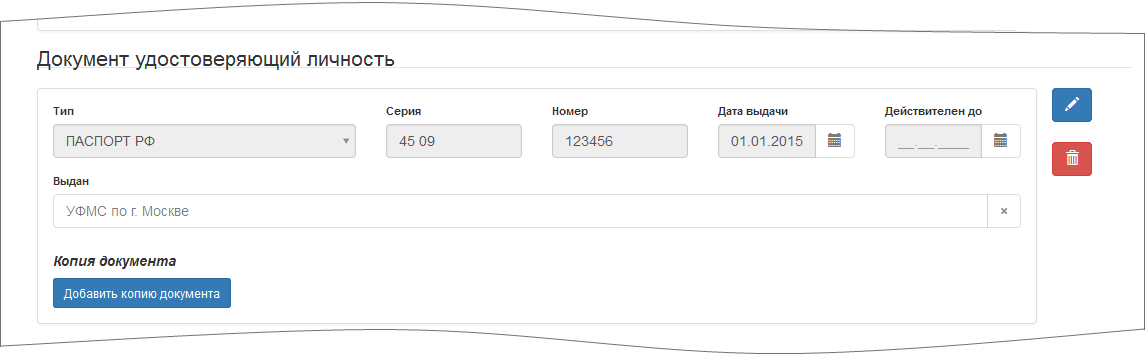
\includegraphics[width = 1\textwidth ,keepaspectratio]{cl_docs}
 \caption{Регистрационная карточка пациента. Блок <<История изменений документов>>}
 \label{img_cl_docs}
\end{figure} 


\subsection{Регистрация нового пациента} \label{cl_new}

Для регистрации нового пациента необходимо в верхней части страницы нажать кнопку \btn{Обслуживание пациентов}, после чего нажать кнопку \btn{Зарегистрировать пациента}  в правой части страницы.

\begin{vnim}
Перед началом регистрации нового пациента необходимо убедиться, что данный пациент не был зарегистрирован ранее. Для этого рекомендуется воспользоваться поиском (см. раздел \ref{cl_find})
\end{vnim}

\begin{vnim}
Если после выполнения поиска пациентов, кнопка регистрации не видна на экране, нужно нажать в поле поиска клавишу \keys{Enter} на клавиатуре.
\end{vnim}
 
После нажатия кнопки \btn{Зарегистрировать пациента} откроется страница регистрационной карточки пациента,  содержащая незаполненные поля. Необходимо ввести все данные пациента в пустые поля в соответствии с разделом \ref{cl_card} Для сохранения введенных данных требуется нажать кнопку \btn{Сохранить} в левой части страницы. Если какие-либо поля регистрационной карточки были заполнены неправильно или некоторые обязательные для заполнения поля остались пустыми, сохранение будет невозможно. При нажатии на кнопку \btn{Сохранить} рядом с кнопкой будет выдаваться соответствующая подсказка.

Если сохранение карточки не требуется, нужно нажать кнопку \btn{Отмена} в левой части страницы.

Перемещение между блоками регистрационной карточки можно выполнять как с помощью полос прокрутки или колесика мыши, так и с помощью ссылок на блоки, расположенных в левой части страницы регистрационной карточки пациента (Рисунок \ref{img_cl_content}). Для того, чтобы перейти к нужному блоку с помощью ссылки, достаточно щелкнуть по ней левой кнопкой мыши.

\begin{figure}[ht]\centering
 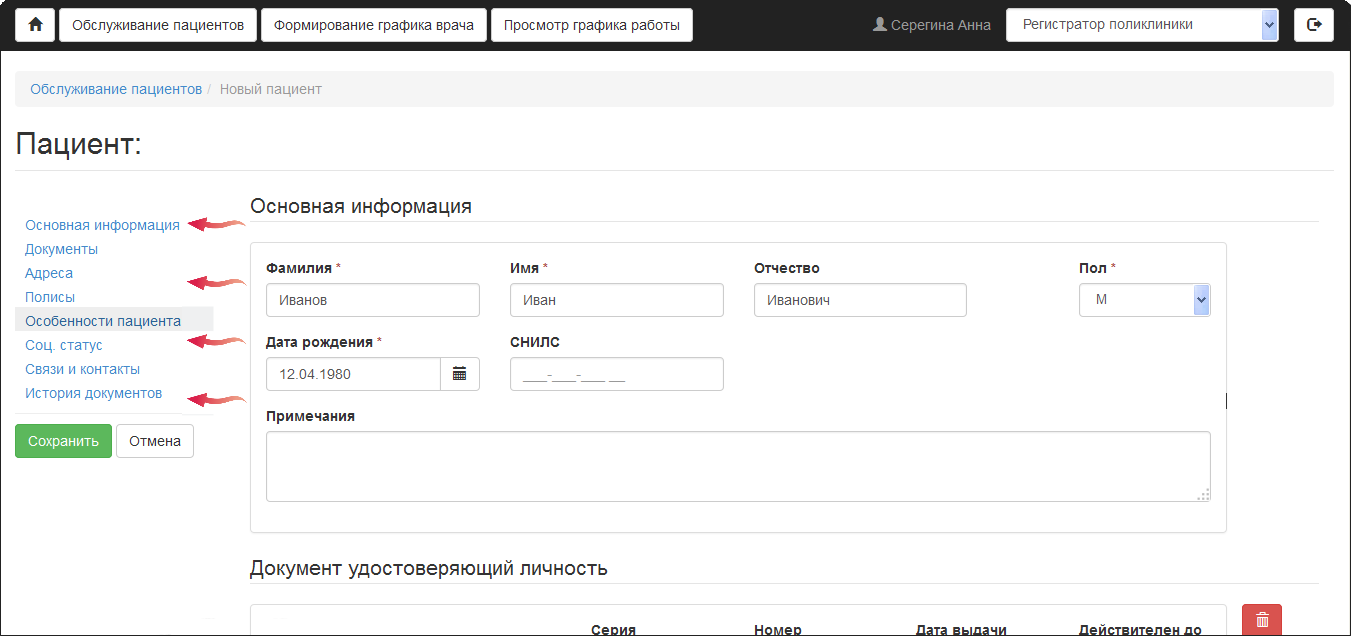
\includegraphics[width = 1\textwidth ,keepaspectratio]{cl_content}
 \caption{Ссылки на блоки регистрационной карточки}
 \label{img_cl_content}
\end{figure} 

\subsection{Редактирование регистрационной карточки пациента}

Данные, введенные в регистрационную карточку пациента, не являются статичными, их можно динамически изменять в соответствии с изменениями первичных документов у пациента. При изменении каких-либо документов у пациента, его социального статуса, выявлении новых особенностей и т.п., требуется открыть регистрационную карточку пациента на редактирование и внести в нее соответствующие изменения. 

Для редактирования регистрационной карточки пациента, следует найти пациента в БД, щелкнуть по записи о пациенте левой кнопкой мыши (Рисунок \ref{img_cl_findrez}) и в открывшемся окне (Рисунок \ref{img_cl_contrwin}) нажать кнопку \btn{Редактировать данные пациента}. Поиск пациентов описан в разделе \ref{cl_find}

\begin{figure}[ht]\centering
 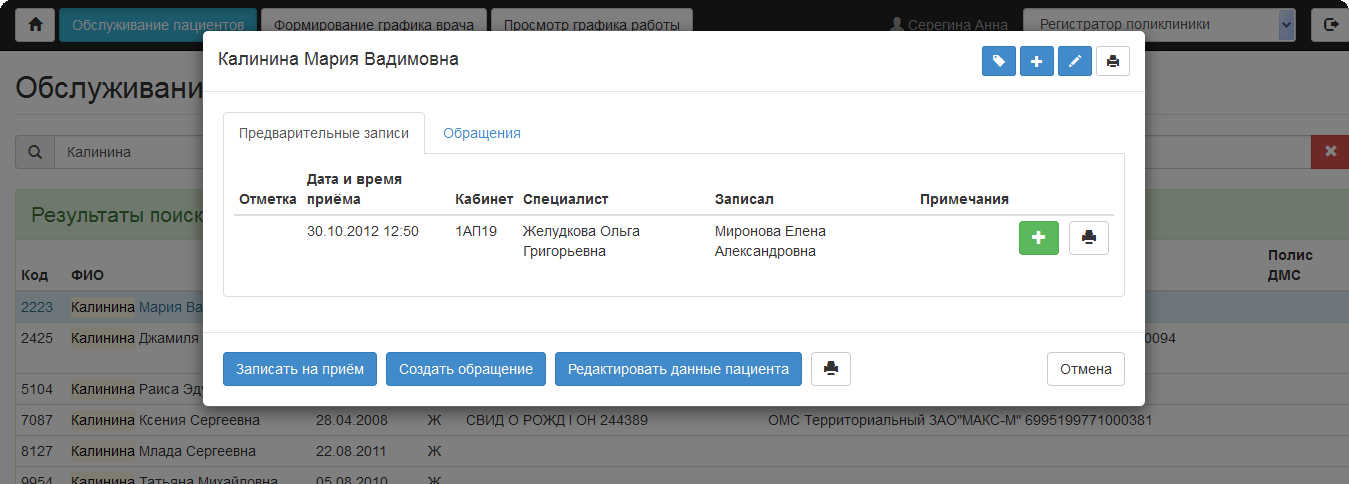
\includegraphics[width = 1\textwidth ,keepaspectratio]{cl_contrwin}
 \caption{Окно управления обслуживанием пациента}
 \label{img_cl_contrwin}
\end{figure} 

Откроется страница, содержащая заполненную регистрационную карточку пациента. Требуется внести изменения в соответствующие поля и сохранить их, нажав кнопку \btn{Сохранить}. Состав полей и методы их заполнения подробно рассмотрены в разделе \ref{cl_card}

Блок редактирования основной информации о пациенте доступен для редактирования постоянно. Для того, чтобы отредактировать любой другой блок, необходимо нажать кнопку 
\includegraphics[scale=0.6]{edt} справа от соответствующего блока или подраздела, после чего поля соответствующего блока станут доступными для редактирования.

Для удаления информации из какого-либо блока или подраздела нужно нажать кнопку 
\includegraphics[scale=0.6]{del} справа от  него. Появится диалоговое окно с запросом подтверждения удаления. Следует нажать кнопку \btn{ОК} в этом окне, после чего информация будет удалена. В блоке \dm{Документ удостоверяющий личность} при удалении все поля очищаются, но не удаляются со страницы. При удалении информации в других блоках, поля записи удаляются.

Кнопка \dm{Добавить новый} в блоках \dm{Адрес регистрации и проживания} и \dm{Медицинские полисы} очищает поля соответствующего подраздела для ввода новых данных. Данные предыдущих полисов при этом сохраняются в истории изменений документов. В остальных разделах данная кнопка создает еще одну запись в выбранном подразделе.

\subsection{Вывод на печать медицинских документов пациента}

Из регистрационной карточки пациента можно распечатать ряд медицинских документов. Для этого требуется нажать кнопку 
\includegraphics[scale=0.6]{print} в правом верхнем углу страницы регистрационной карточки пациента. Откроется окно \dm{Печать документов}, содержащее список доступных печатных форм (Рисунок \ref{img_cl_printm}). Флажками слева от названия отмечаются документы, выбранные для отправки на печать. Нужно снять флажки с названий документов, которые печатать не требуется, и нажать кнопку \btn{Печать}. Отмеченные флажками документы будут отправлены на принтер.

\begin{figure}[ht]\centering
 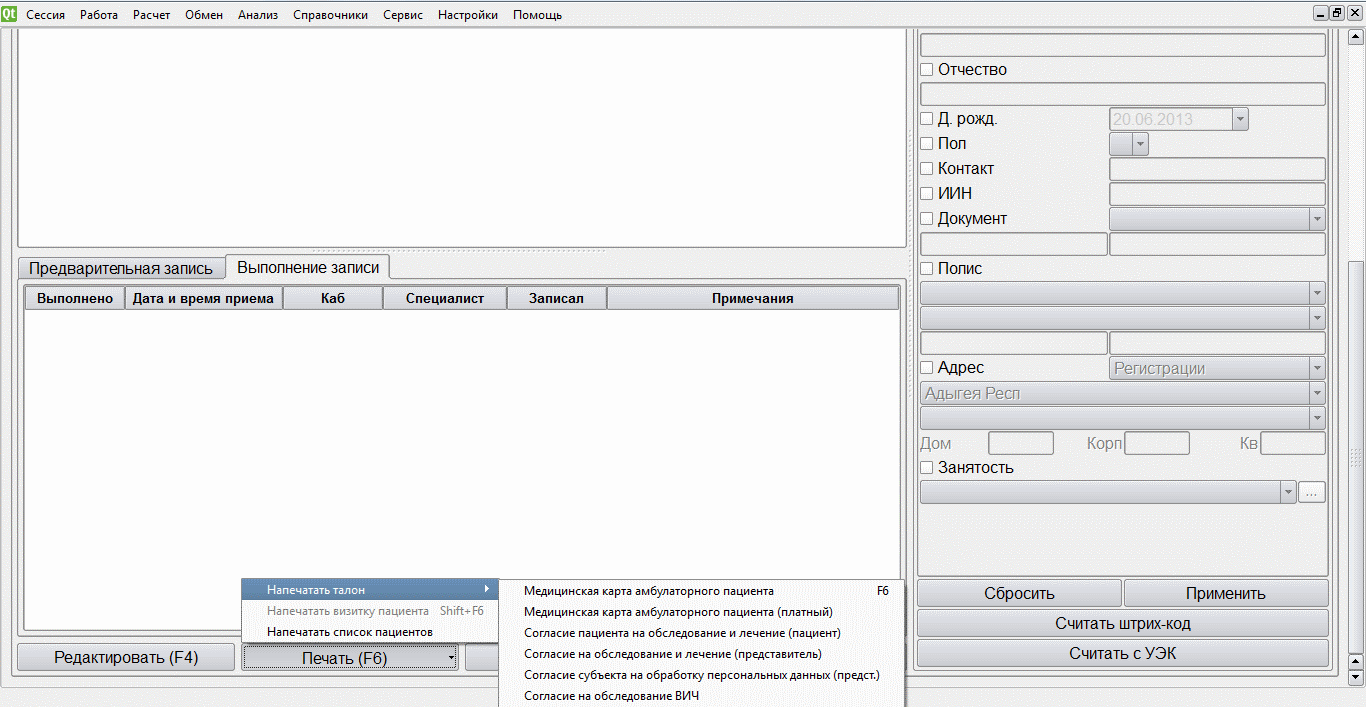
\includegraphics[width = 1\textwidth ,keepaspectratio]{cl_printm}
 \caption{Печать медицинских документов пациента}
 \label{img_cl_printm}
\end{figure} 

Кнопка \btn{Печать компактно} тоже выводит выбранные документы на печать, но не делает переход на новую страницу для каждого нового дукумента.

Печать документов пациента так же можно вызвать со страницы обслуживания пациентов (Рисунок \ref{img_cl_findrez}). Для этого необходимо найти пациента и щелкнуть по нему левой кнопкой мыши. В открывшемся окне (Рисунок \ref{img_cl_contrwin}) нужно нажать кнопку 
\includegraphics[scale=0.6]{print} в нижней части либо в правом верхнем углу окна. Откроется список документов для печати (Рисунок \ref{img_cl_printm}), где можно выбрать и вывести на печать документы вышеописанным способом. 
   
Печать медицинских документов, создаваемых в процессе обследования и лечения пациента, будет рассмотрена в следующих разделах.

